\documentclass[a4paper]{scrreprt}

\usepackage[german]{babel}
\usepackage[utf8]{inputenc}
\usepackage[T1]{fontenc}
\usepackage{ae}
\usepackage[bookmarks,bookmarksnumbered]{hyperref}
\usepackage{graphicx}
\usepackage[toc]{glossaries}
\usepackage{float}
\usepackage{listings}

\graphicspath{ {Images/} }
\setcounter{secnumdepth}{5}
\makeglossaries

\begin{document}
    \def\code#1{\texttt{#1}}

    \begin{flushright}
        
\includegraphics[scale = 0.7]{kit-logo.jpg}\\[0.5cm]
        % 
\includegraphics[scale = 1]{teco.jpg}
    \end{flushright}
    % 
\includegraphics[scale = 0.5]{kit-logo.jpg} \hspace{4cm} 
\includegraphics[scale = 1]{teco.jpg}
    \vspace*{2cm}

    \begin{center} \large

        Praxis der Softwareentwicklung
        \vspace * {1.5cm}

        \textbf{\huge Mind Rate}

        \vspace*{1cm}


        {\Large Ein interaktives System mit Android-Client f\"ur Studien nach Experience-Sampling-Method (ESM)}

        \vspace*{1cm}

        \textbf{\Large Entwurf}
        \vspace*{2cm}

        Shanshan Du, Yi Ge, Renhan Lou, Ruoheng Ma, Haobin Tan
        \vspace*{1cm}

        02. Dezember 2016
        \vspace*{2.5cm}

        Betreuung: Anja Exler, Dr. Andrea Schankin\\[0.5cm]
        Forschungsgruppe TECO: Technology for Pervasive Computing\\[0.5cm]

        Karlsruher Institut für Technologie
    \end{center}
    \thispagestyle{empty}

    \tableofcontents

    \chapter{Allgemeine Struktur}

        Der Entwurf besteht aus zwei Seiten: der Android-App-Seite und der Server-Seite. Sie sind jeweils für die Android-App und das Web-Interface verantwortlich. Zusätzlich soll eine Datenbank auf dem Server laufen, um alle Studien-, Konto- und Probandendaten zu speichern. Diese gehört auch zu der Server-Seite. Die zwei Seiten sollen miteinander durch das HTTP-Protokoll kommunizieren.

    \chapter{Server-Seite}
        Die Server-Seite nutzt eine von Django-Framework veränderte Variante\footnote{\href{https://docs.djangoproject.com/en/1.10/faq/general/\#django-appears-to-be-a-mvc-framework-but-you-call-the-controller-the-view-and-the-view-the-template-how-come-you-don-t-use-the-standard-names}{https://docs.djangoproject.com/en/1.10/faq/general/\#django-appears-to-be-a-mvc-framework-but-you-call-the-controller-the-view-and-the-view-the-template-how-come-you-don-t-use-the-standard-names}} der Modell-Präsentation-Steuerung-Architektur (MVC) als den Architekturstil. Die benötigte Klassen werden als Modelle entworfen. Der Entwurf von Server-Seite wird auf Python angefertigt.

        \section{Modelle}
            \begin{itemize}
                \item \code{class StudyDirector}
                    \begin{itemize}
                        \item \code{studies = []: Study}
                        \item \code{surname}
                        \item \code{firstName}
                        \item \code{mailAddress}
                    \end{itemize}

                    \item \code{class Study}
                        \begin{itemize}
                            \item \code{probands = []: Proband}
                            \item \code{id}
                            \item \code{name}
                            \item \code{beginningDate}
                            \item \code{endDate}
                            \item \code{director: StudyDirector}
                            \item \code{questionnaires = []: Questionnaire}
                        \end{itemize}

                    \item \code{class Proband}
                        \begin{itemize}
                            \item \code{study: Study}
                            \item \code{id}
                            \item \code{birthday}
                            \item \code{occupation}
                            \item \code{gender}
                        \end{itemize}

                    \item \code{class Questionnairer}
                        \begin{itemize}
                            \item \code{questions = []: AbstractQuestion}
                            \item \code{id}
                            \item \code{name}
                            \item \code{study: Study}
                            \item \code{triggerEvent: TriggerEvent}
                            \item \code{answeringTime}
                            \item \code{answers = []: QuestionnaireAnswer}
                        \end{itemize}

                    \item \code{class QuestionnaireAnswer}
                        \begin{itemize}
                            \item \code{submitter: Proband}
                            \item \code{submitTime}
                            \item \code{questionAnswers = []: AbstractQuestionAnswer}
                        \end{itemize}

                    \item \code{class AbstractQuestion(ABC)}
                        \begin{itemize}
                            \item \code{id}
                            \item \code{questionnaire: Questionnaire}
                        \end{itemize}

                    \item \code{class TextQuestion(AbstractQuestion)}
                        \begin{itemize}
                            \item \code{content}
                        \end{itemize}

                    \item \code{class ChoiceQuestion(AbstractQuestion)}
                        \par // Both single choice question and multiple choice question are belonging to this class.
                        \begin{itemize}
                            \item \code{options = \{\}}
                            \item \code{followUpQuestion: AbstractQuestion}
                            \item \code{followUpQuestionTriggerOptions = []}
                        \end{itemize}

                    \item \code{class SteplessScaleQuestion(AbstractQuestion)}
                        \par // Scale questions with steps are effectively just single choice questions; therefore they are not a class.
                        \begin{itemize}
                            \item \code{scaleMin: int}
                            \item \code{scaleMax: int}
                            \item \code{followUpQuestion: AbstractQuestion}
                            \item \code{followUpQuestionTriggerMin: int}
                            \item \code{followUpQuestionTriggerMax: int}
                        \end{itemize}

                    \item \code{class AbstractQuestionAnswer(ABC)}
                        \begin{itemize}
                            \item \code{content}
                        \end{itemize}

                   \item \code{class TextQuestionAnswer(AbstractQuestionAnswer)}
                       \begin{itemize}
                           \item \code{content: string}
                       \end{itemize}

                   \item \code{class MultiChoiceQuestionAnswer(AbstractQuestionAnswer)}
                       \begin{itemize}
                           \item \code{content = []: string}
                       \end{itemize}

                    \item \code{class SingleChoiceQuestionAnswer(AbstractQuestionAnswer)}
                        \begin{itemize}
                            \item \code{content: string}
                        \end{itemize}

                    \item \code{class SteplessScaleQuestionAnswer(AbstractQuestionAnswer)}
                        \begin{itemize}
                            \item \code{content: int}
                        \end{itemize}

            \end{itemize}

        \newpage
        \section{Entity-Relationship-Modell der Datenbank}
            \begin{figure}[ht]
                \centering
                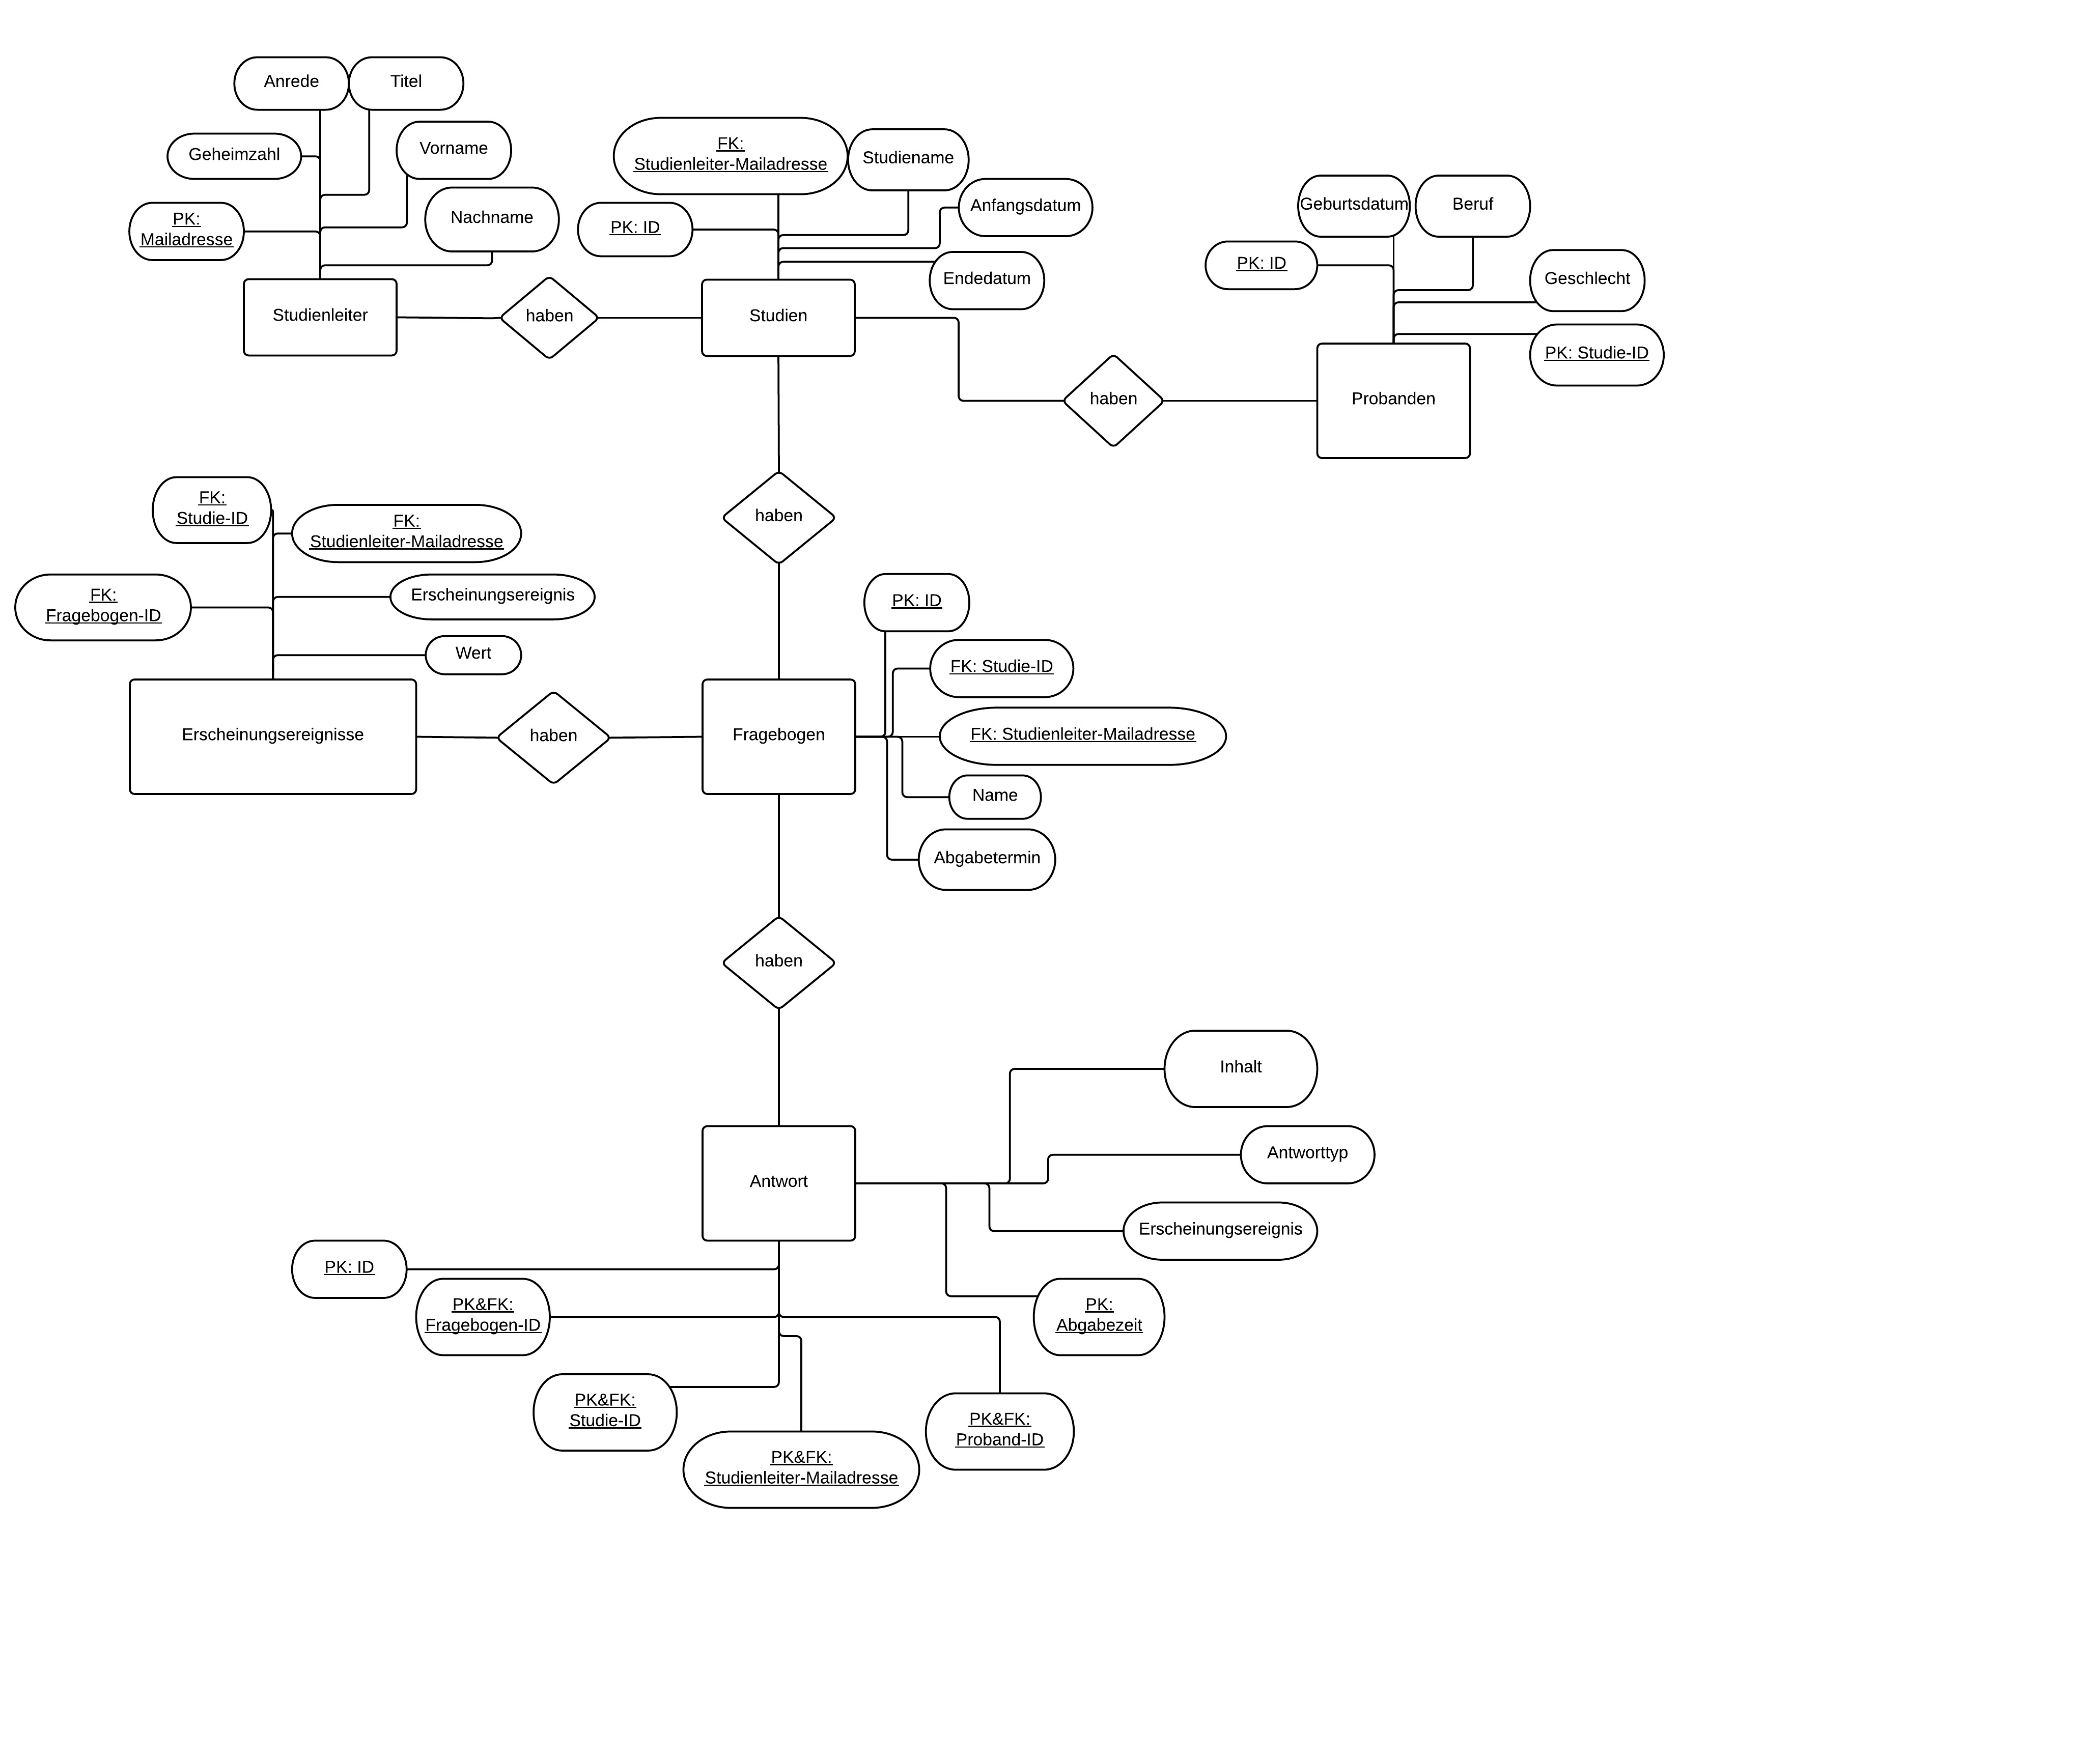
\includegraphics[scale = 0.13]{PSE_Datenbank_ERM.jpeg}
                \caption{Entity-Relationship-Modell der Datenbank}
            \end{figure}


    \newpage
    \chapter{Android-App}

        Das Entwurfsmuster Model View Controller (MVC, englisch für Modell-Präsentation-Steuerung) wird hier eingesetzt, um einen fleixbler Programmentwurf zu ermöglichen.


        \vspace*{1cm}
        \section{Überblick von Pakete}

            Das folgende Diagramm dient sich als einen Überblick über unsere Android App. Modell, Präsentation udn Steuerung werden mit drei verschiedenen Farbe dargestellt: blau für Modell, grün für Präsentation und gelb für Steuerung.

            \noindent Um die Beziehungen zwischen Klassen und das System ganzheitlich aufzufassen, enthält folgendes Diagramm keine Attribute und Methoden. Jede Pakete sowie Klasse mit Attribute und Methoden werden dann ausführlich beschreiben.



            \newpage
            \vspace*{1cm}
            \begin{figure}[H]
                \centering
                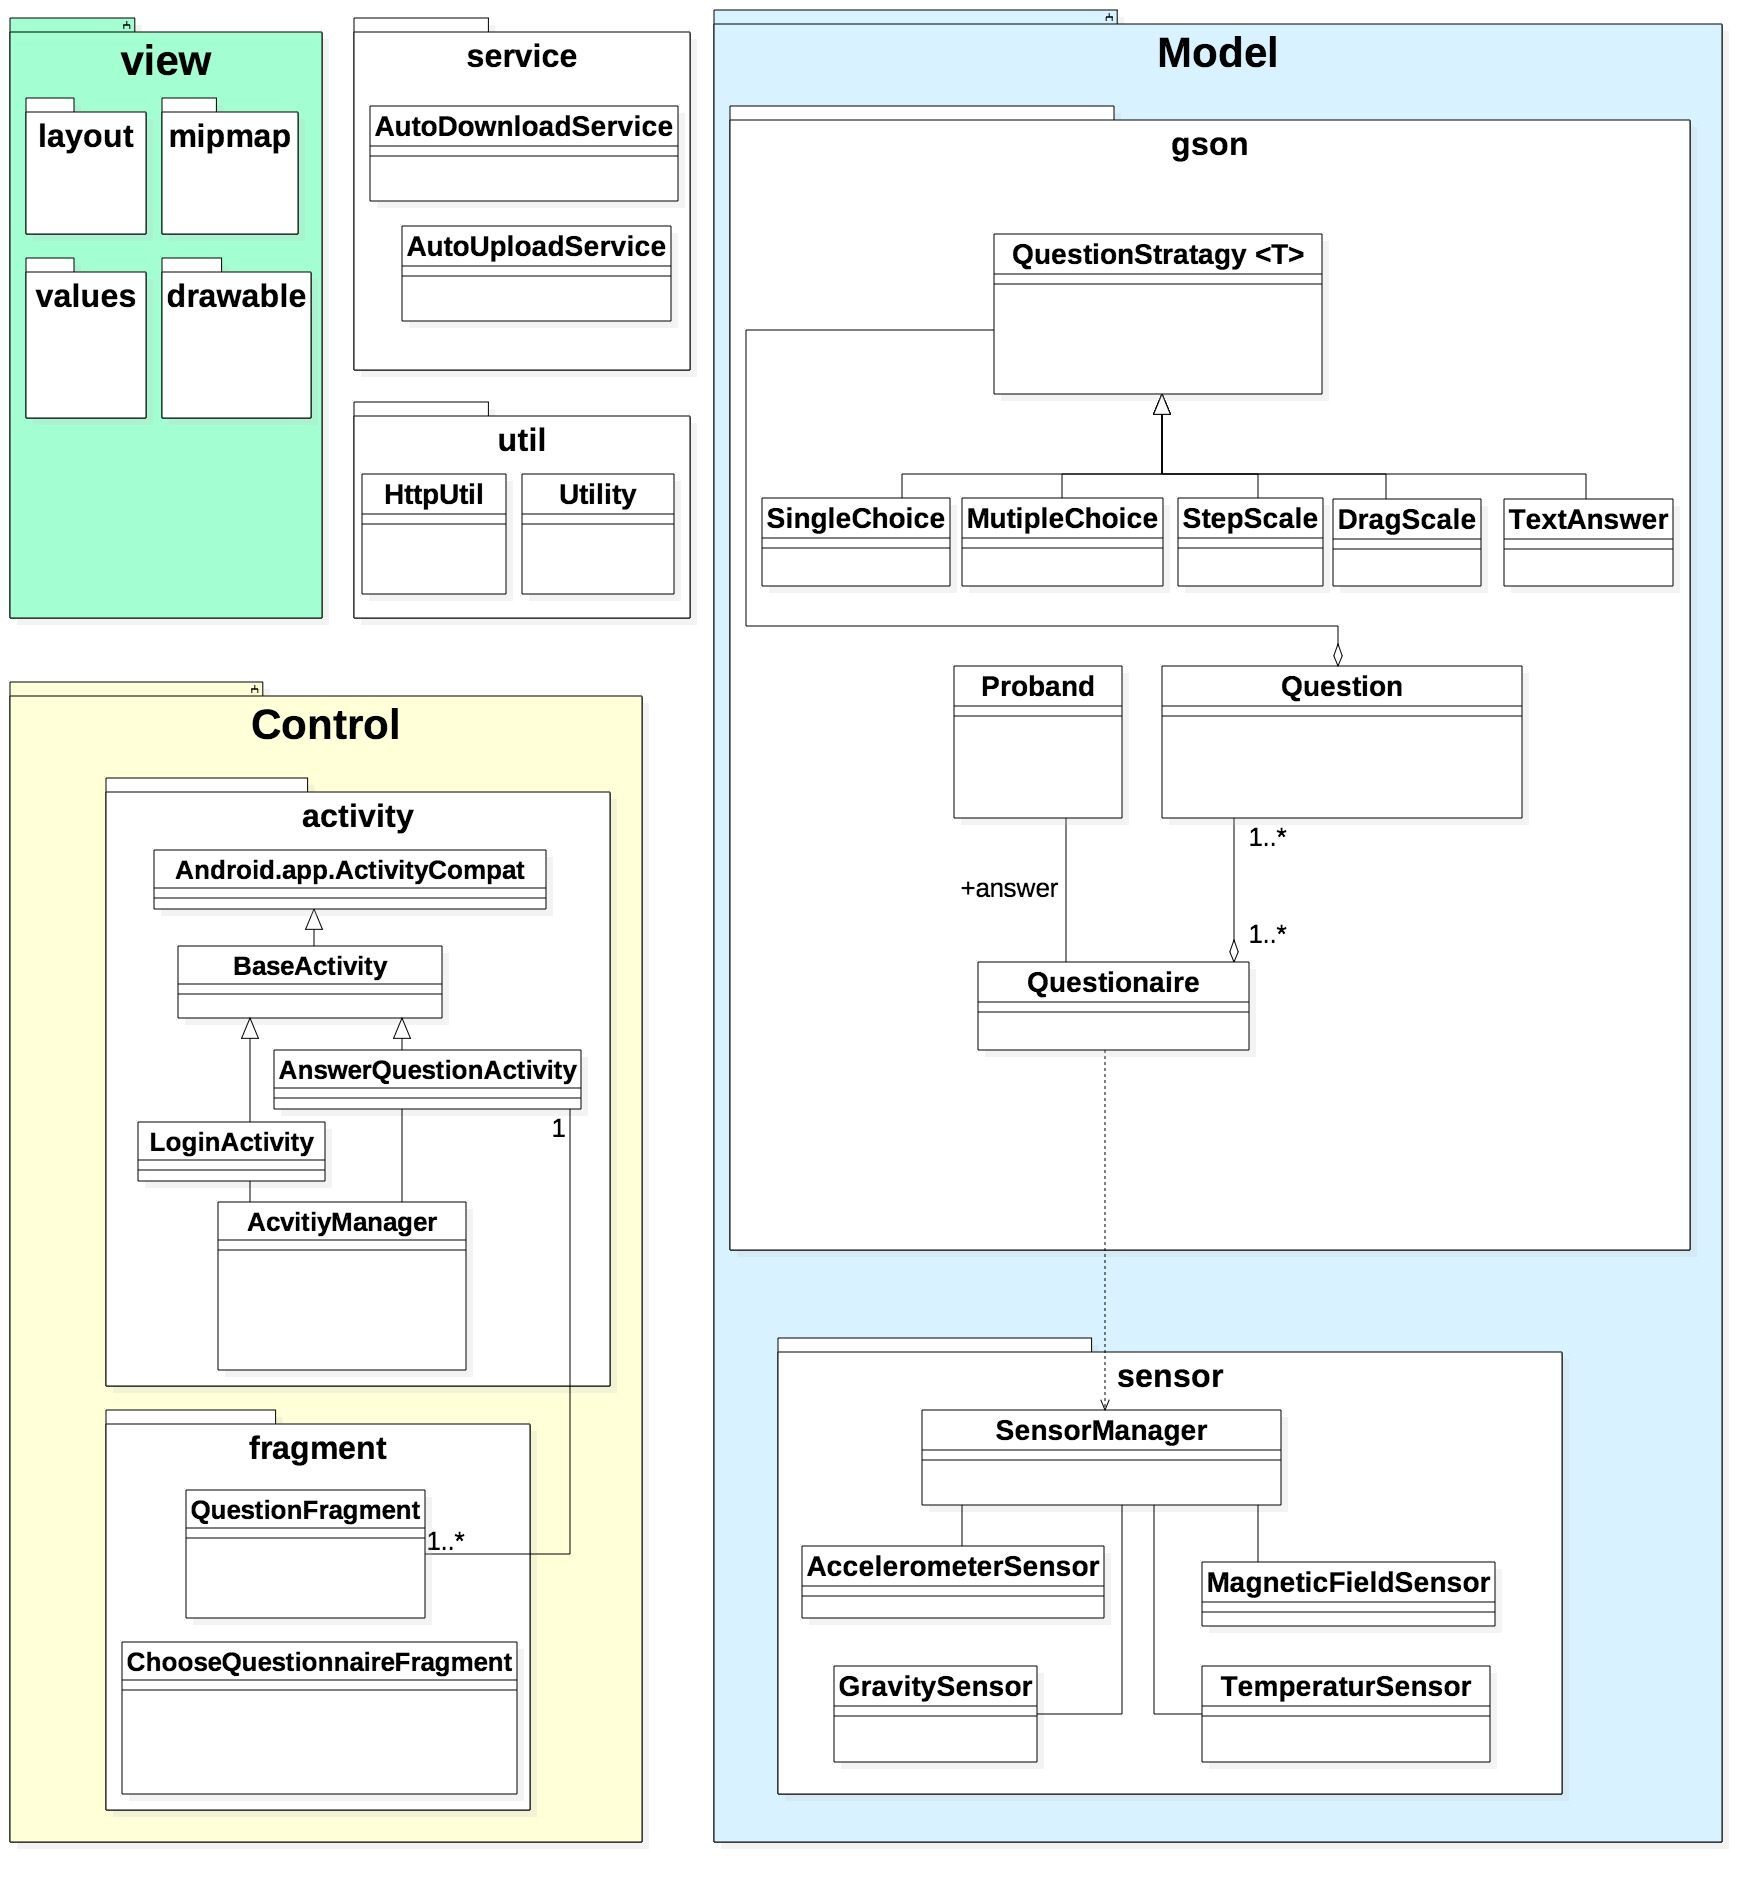
\includegraphics[scale = 0.25]{packageDiagram.jpg}
                \caption{Überblick über alle Packte und Klasse (ohne Attribute und Methoden)}
            \end{figure}




        %TODO: Ausführliche Beschreibung für jedes package und klasse davon

        \section{Model}

            Der Teil Model besteht aus zwei Pakete: gson und sensor.

            \begin{figure}[H]
                \centering
                % 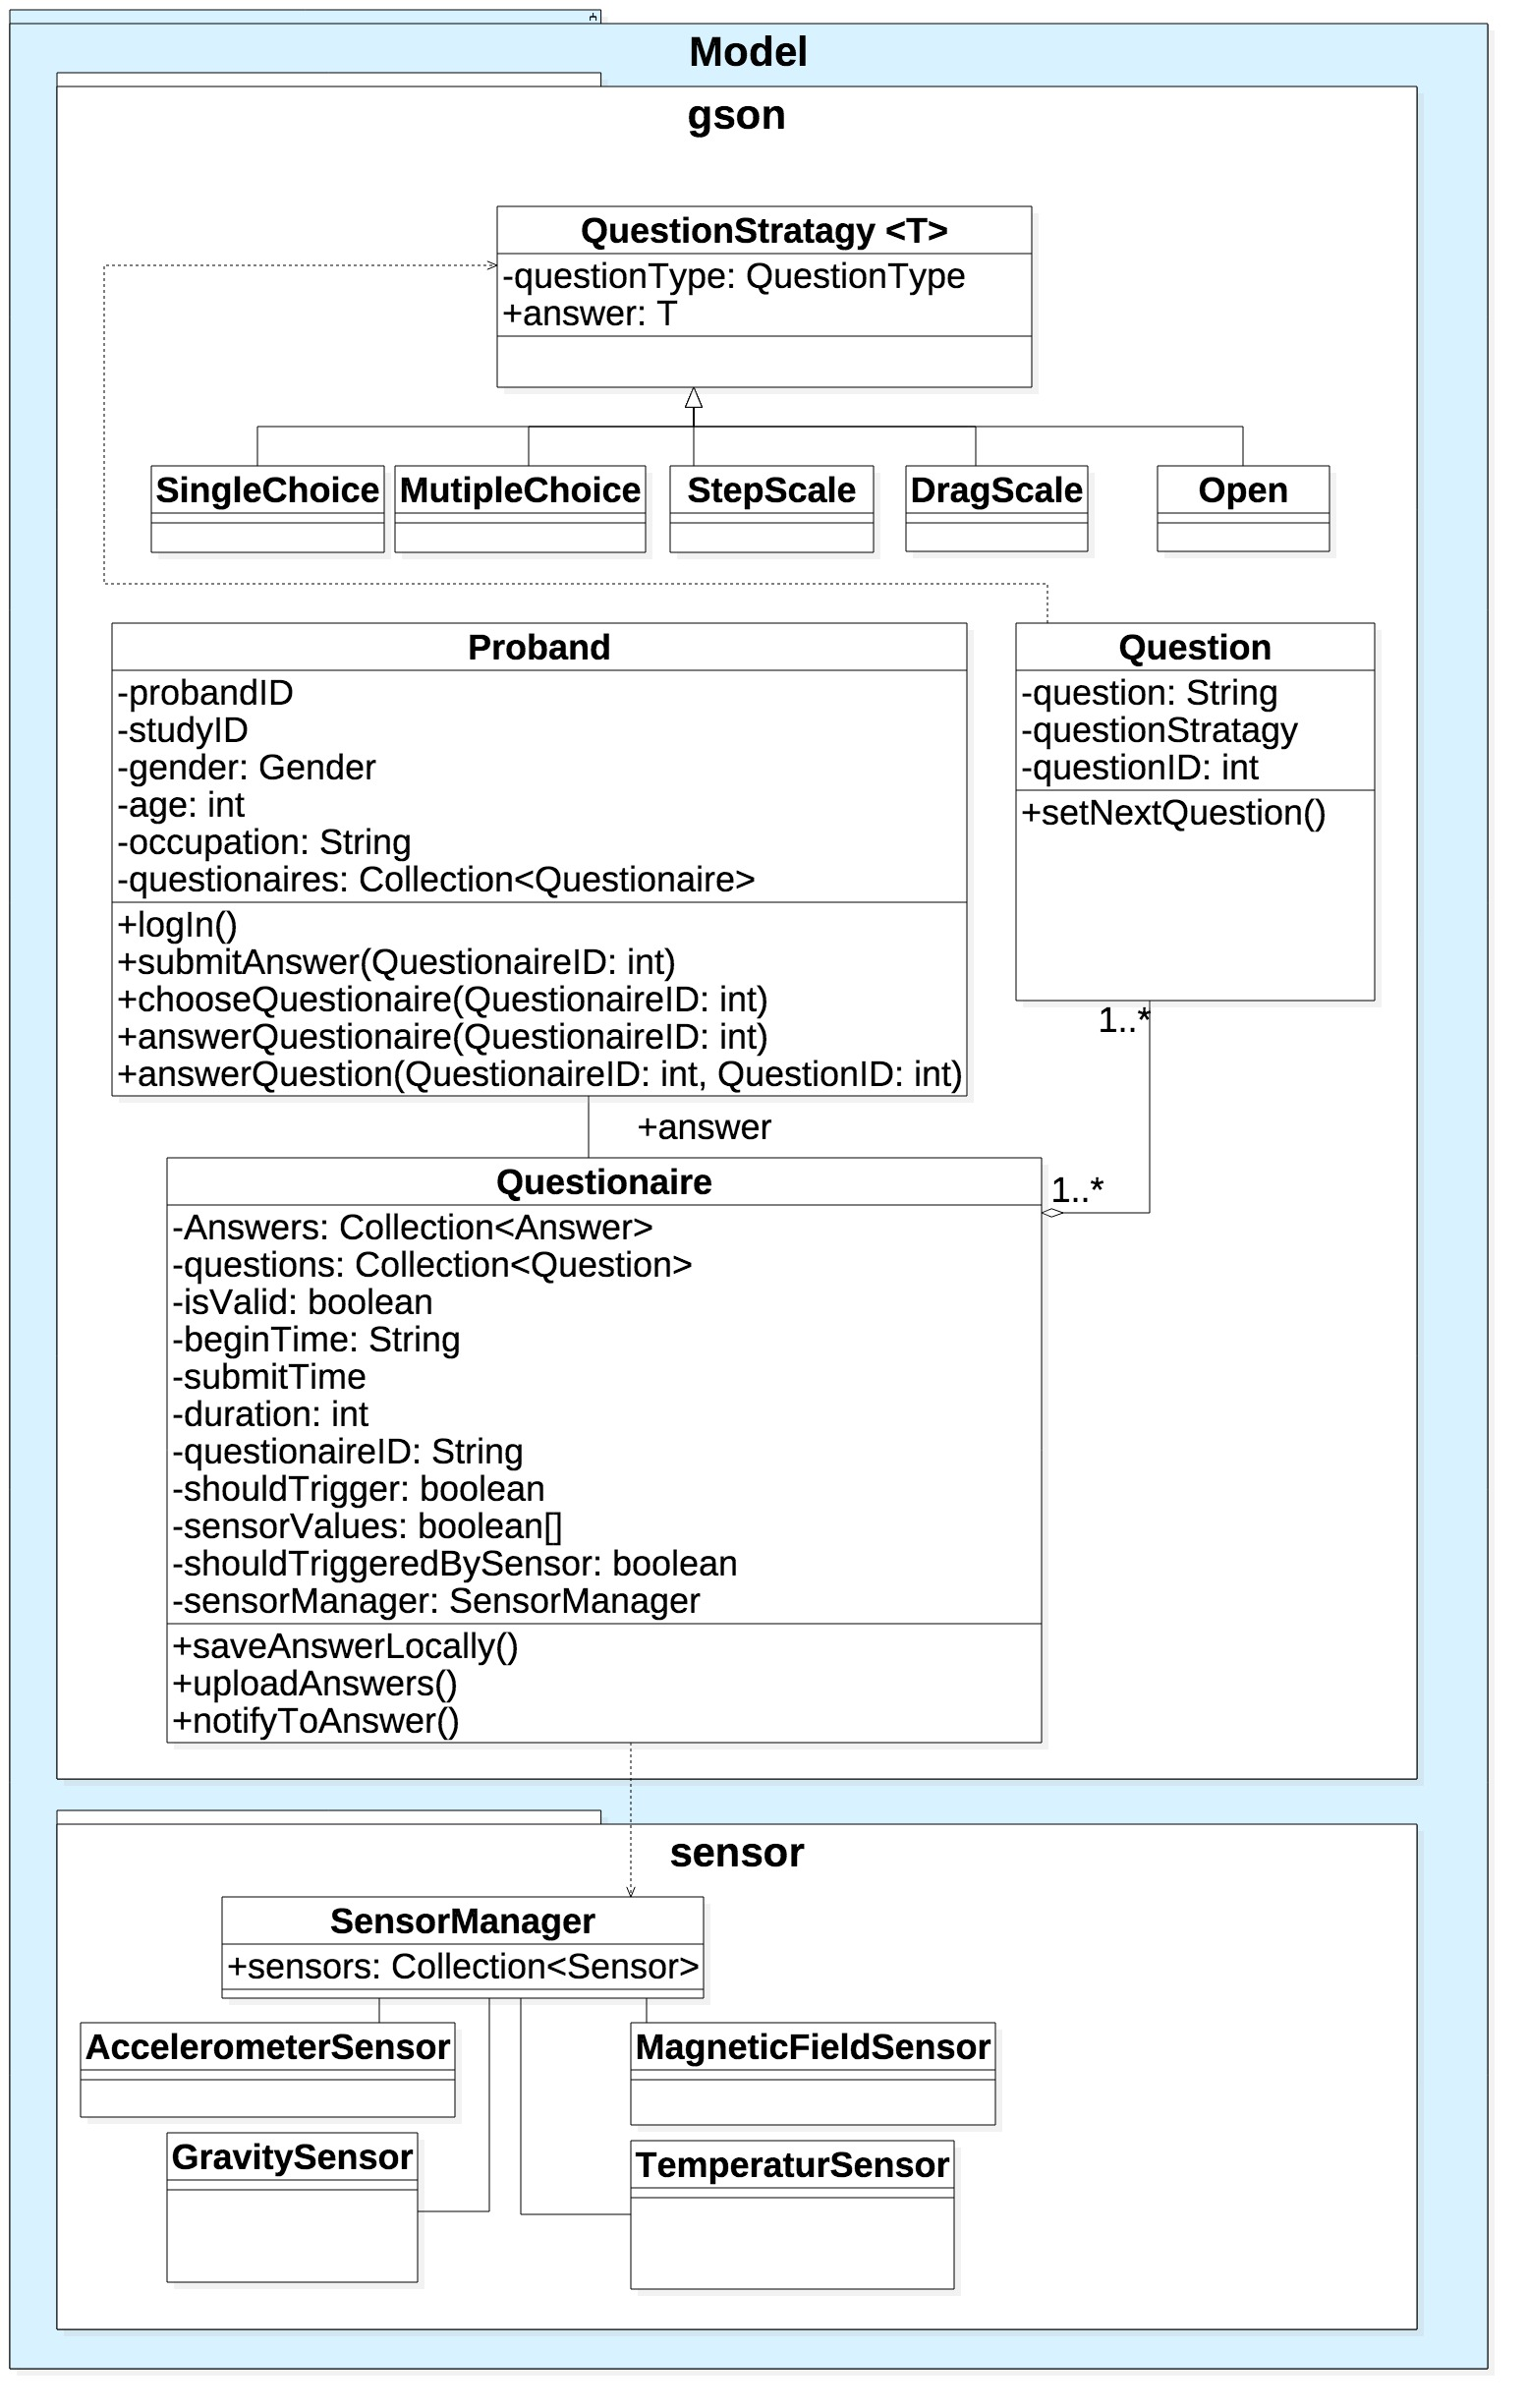
\includegraphics[scale = 0.25]{Model.jpg}
                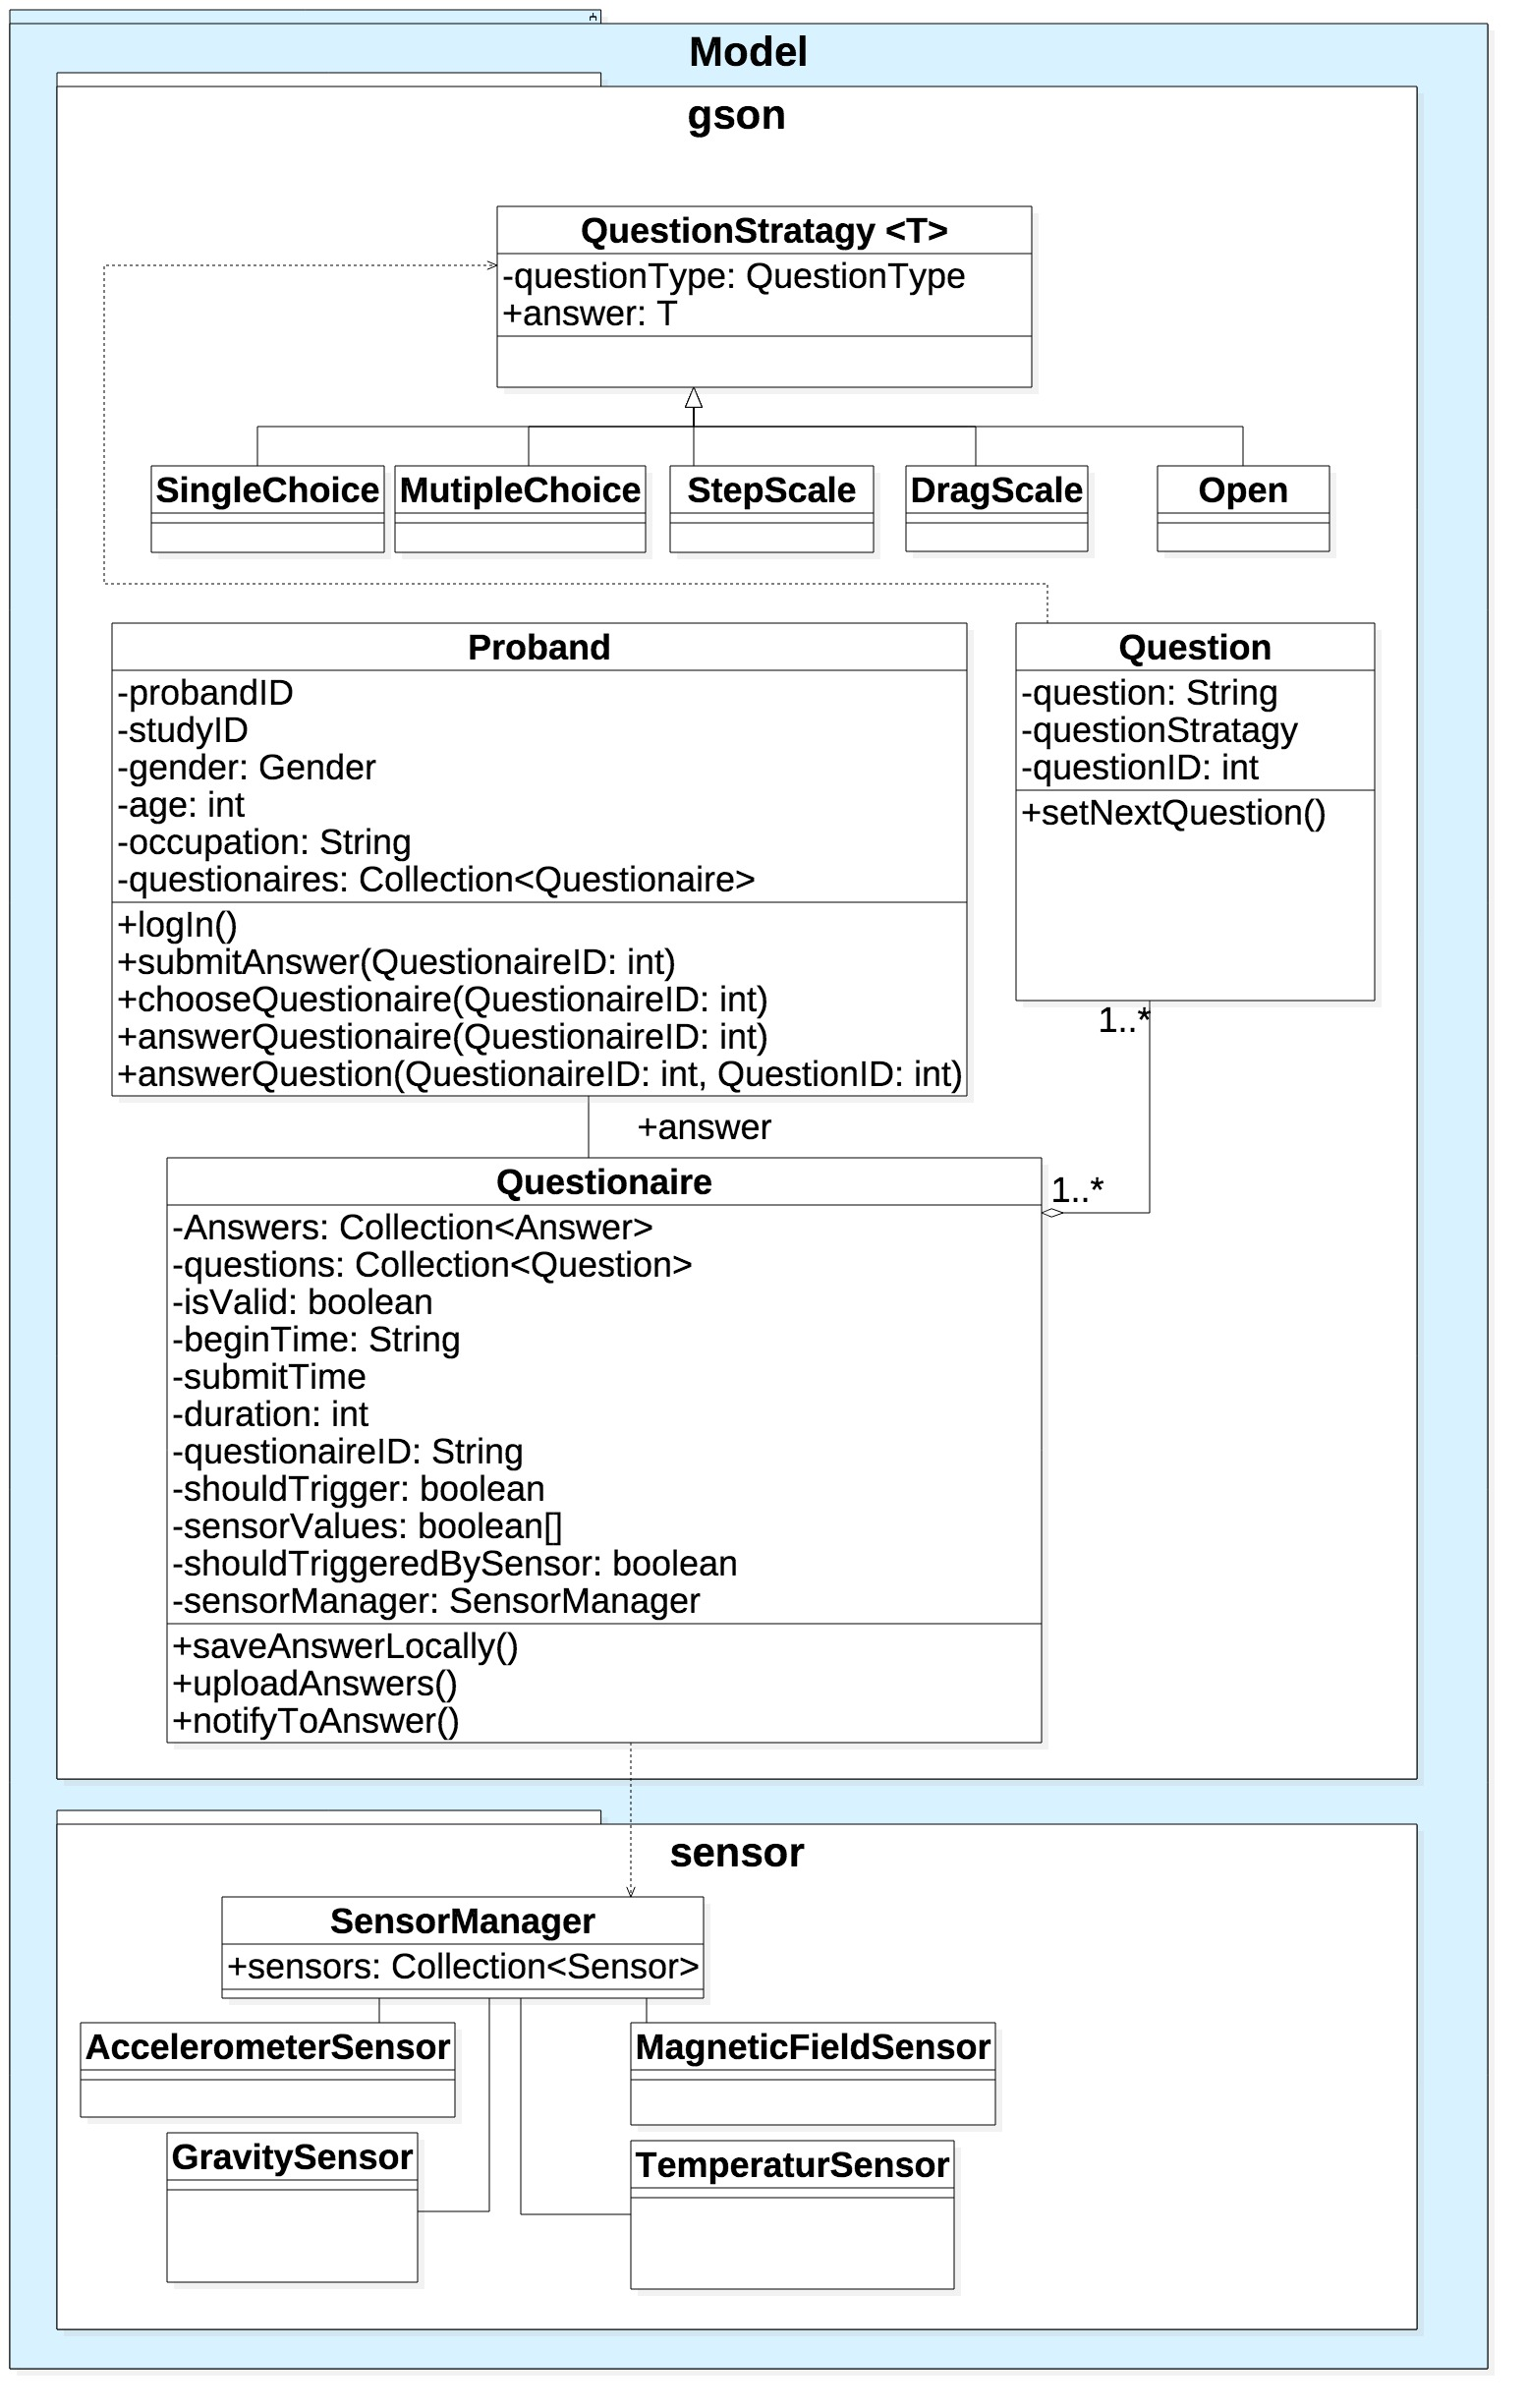
\includegraphics[scale=0.28]{Model.jpg}
                \caption{Model (Modelle)}
            \end{figure}


            \newpage
            \subsection{gson}



                \subsubsection{Proband}


                    % \begin{listing}[language=Java]
                    %     public class Proband {
                        
                    %     }
                    % \end{listing}

                \subsubsection{Questionnaire}

                \subsubsection{Question}

                \subsubsection{QuestionStrategy} %super abstract class
                    \begin{itemize}
                        \item SingleChoice
                        \item MultiChoice
                        \item StepScale
                        \item DragScale
                        \item TextAnswer
                    \end{itemize}

            \subsection{Sensor}

                \subsubsection{SensorManager}
                \subsubsection{AccelerometerSensor}
                \subsubsection{GravitySensor}
                \subsubsection{MagneticFeldSensor}
                \subsubsection{TemperatureSensor}


        \section{View}

            % provided by android


        \section{Control}
            \begin{figure}[H]
                \centering
                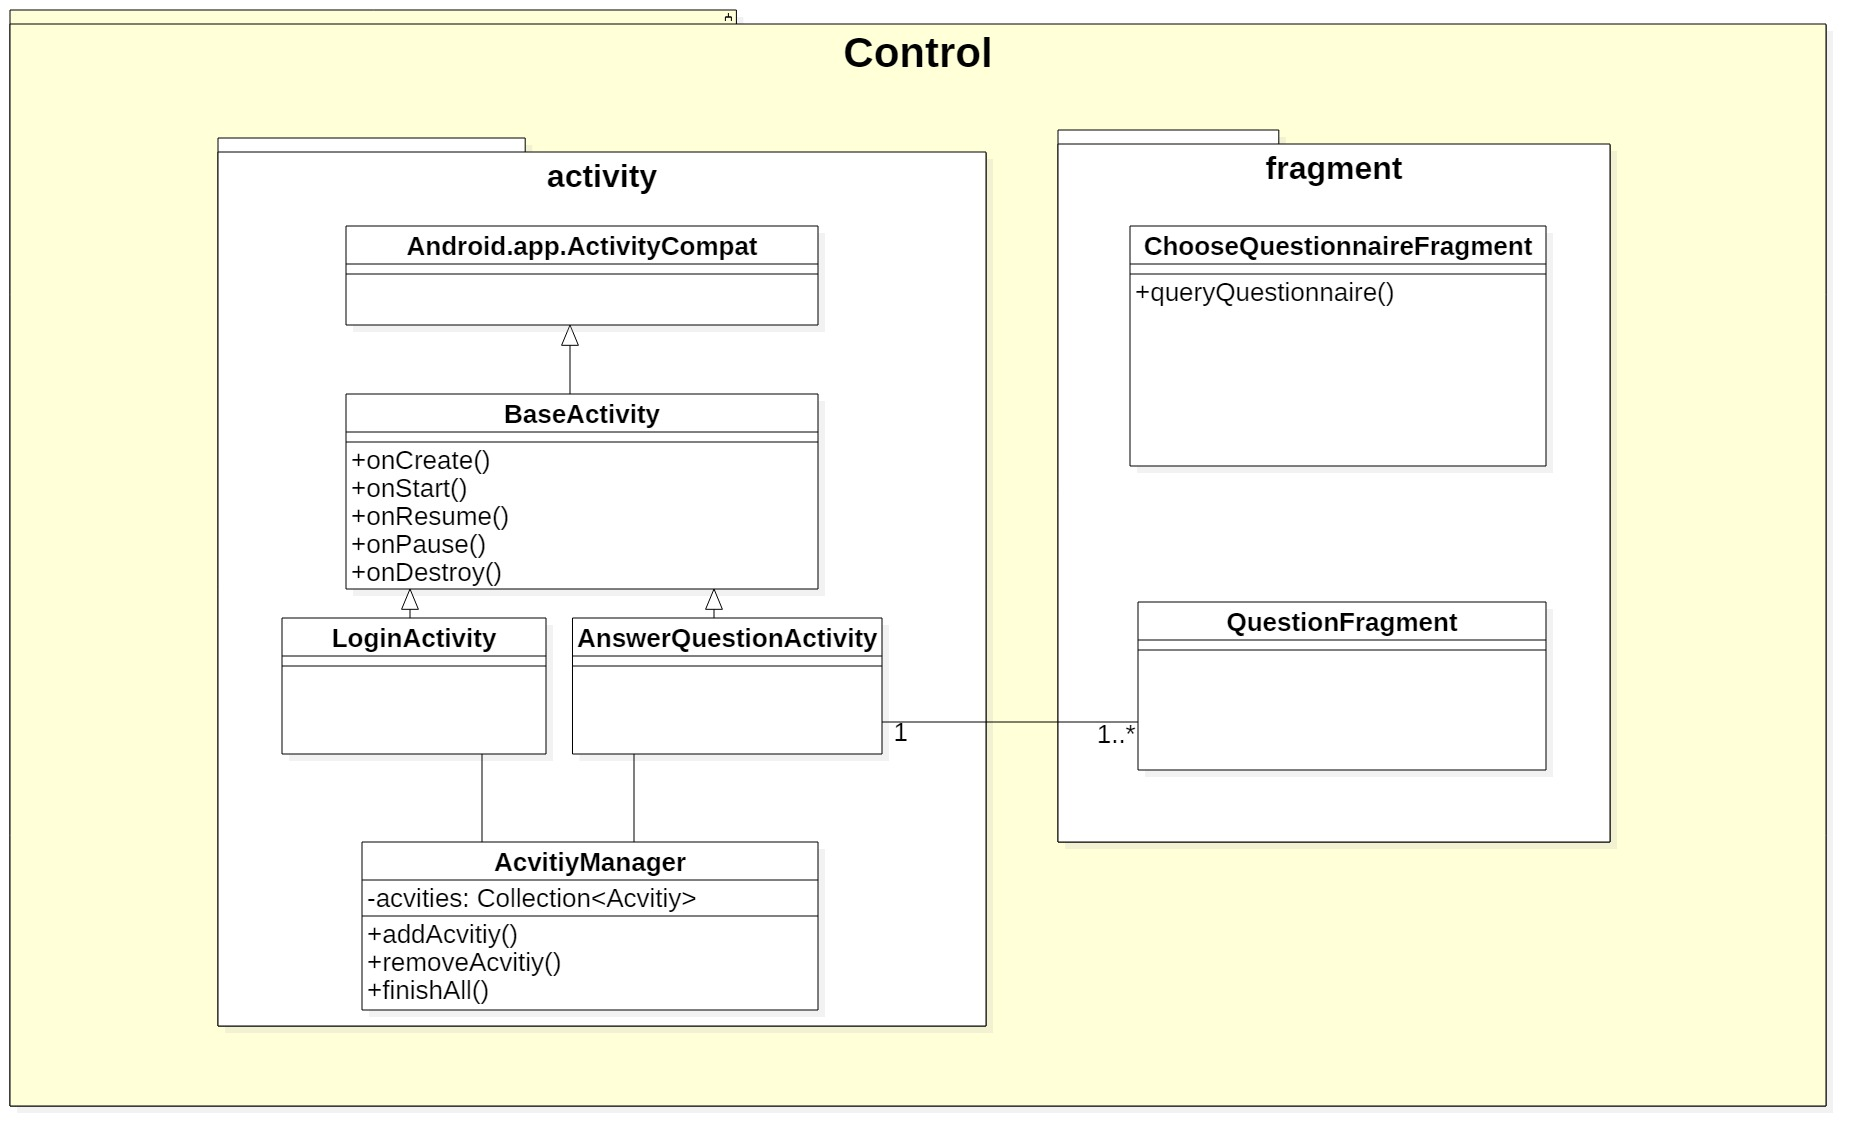
\includegraphics[scale = 0.25]{ControlClassDiagram(Android).jpg}
                \caption{Klassendiagramm für Control in der Android Applikation }
            \end{figure}
            \subsection{activity}

                \subsubsection{ActivityManager}
                \subsubsection{BaseActivity}
                \subsubsection{LogInActivity}
                \subsubsection{AnswerQuestionActivity}

            \subsection{fragment}

                \subsubsection{ChooseQuestionnaireFragment}
                \subsubsection{QuestionFragment}

        \section{HilfPaket}

            \subsection{service}

                \subsubsection{AutoDownloadService}

                \subsubsection{AutoUploadService}

            \subsection{util}

                \subsubsection{HttpUtil}

                \subsubsection{Util}

    \glsaddall
    \printglossary

    % Abbildungsverzeichnis
    \listoffigures

\end{document}
